\section{Trasformata zeta}
La trasformata zeta aiuta l'analisi di stabilità e causalità delle frequenze dei sistemi lineari a tempo invariante con i relativi filtri, essendo più ampia rispetto alla trasformata di Fourier. 

La trasformata discreta non è sufficiente in alcune situazioni perché non sempre esiste, descrive solo comportamenti di sistemi LTI scarichi e presume condizioni iniziali nulle.

La trasformata zeta è la parte discreta (digitale) della trasformata di Laplace, ed è rappresentata da una sommatoria con l'estensione delle frequenze nel mondo complesso, esprimibile in coordinate polari con un termine $\rho$ qualsiasi che determina la distanza dall'origine. L'operatore è lineare.

\begin{wrapfigure}{R}{0.4\textwidth}
	\vspace{-15pt}
	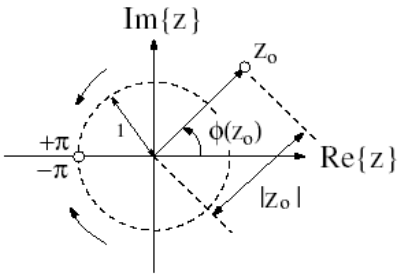
\includegraphics[width=0.4\textwidth]{Lezioni/Immagini/zeta}
	\vspace{-40pt}
\end{wrapfigure}

Data una frequenza bilatera $x(n)$ con $-\infty < n < \infty$ si definisce trasformata zeta:
$$X(z) = Z[x(n)] = \sum_{-\infty}^{\infty} x(n)z^{-n}$$
Esiste una corrispondenza biunivoca tra $x(z)$ e $x(n)$ e i loro domini solo se viene definita la regione di convergenza uniforme ROC, cioè i valori della variabile complessa $z$ tale che $x(z)$ è finita.

Nella regione di convergenza, $X(z)$ è una funzione analitica, cioè continua e indefinitamente derivabile con derivate continue in $z$.

La $z$ è una pulsazione complessa con dominio $\mathcal{C}$, rappresentabile in termini di modulo e fase come $z = \rho e^{j2\pi f} = \rho e^{j\omega}$. Si può ridurre a trasformata di Fourier discreta togliendo il coefficiente complesso e applicando la formula a una nuova sequenza. 

Deve valere la condizione di sommabilità in modulo, quindi la convergenza varia con la distanza e il piano si può dividere in circonferenze concentriche con comportamento diverso. 

La regione ROC dipende solo dal modulo $\rho$ delle pulsazioni complesse $z$, e non dalla loro fase: questo comporta le circonferenze come luoghi dei punti $z$ a modulo costante.
$$ \sum_{-\infty}^{\infty}\abs{x(n)\rho^{-n}} < \infty \implies  \sum_{-\infty}^{\infty}\abs{x(n)}\rho^{-n} < \infty$$
In particolare, è importante trovare i valori di $\rho$ che indicano la convergenza, e si ha che i valori sulla circonferenza di raggio unitario $\rho = 1$ sono i valori della trasformata di Fourier di frequenza 0. Quando c'è un ritardo, la regione sarà individuata con $[z \neq 0]$.

\subsection{Trasformate e ROC}
La trasformata zeta definisce una relazione biunivoca tra la sequenza $x(n)$ e una funzione della variabile complessa $z$. La biunivocità è garantita solo se si specifica la ROC di $X(z)$ e l'espressione analitica della trasformata.

Esistono relazioni specifiche tra la tipologia di una generica sequenza $x(n)$ e la ROC della relativa trasformata $z$:
\begin{itemize}
	\item Le sequenze $x(n)$ bilatere hanno supporto su istanti di tempo discreto negativi e positivi;
	\item Le sequenze causali possiedono coefficienti identicamente nulli per istanti di tempo negativi;
	\item Le sequenze anticausali possiedono coefficienti identicamente nulli per istanti di tempo positivi.
\end{itemize}

\subsubsection{Impulso $\delta$}
$$X(z) = \sum_{-\infty}^{\infty} \delta(n) z^{-n} = 1$$
Se l'impulso $x(n) = \delta(n)$ è una costante nel dominio trasformato, applicando la funzione zeta si ha un risultato simile: tutti i valori assumono 0 tranne quello per cui $n = 0$, quindi l'esponenziale diventa 1 così come tutta la trasformata. 

La regione di convergenza è costante e limitata a 1, e rappresenta tutto il piano complesso per cui la serie geometrica converge.
$$x(n) = 2\delta(n+1) + \delta(n) + 4\delta(n-2) = 2\sum_{-\infty}^{\infty}2\delta(n+1)z^{-n} + \sum_{-\infty}^{\infty}2\delta(n)z^{-n} + 4\sum_{-\infty}^{\infty}2\delta(n-2)z^{-n}$$
$$\implies 2z + 1 + 4z^{-2}$$
Il risultato è ottenuto scomponendo le sommatorie e trovando i valori per cui il numero all'interno delle parentesi si annulla. Bisogna sempre tenere conto del segno negativo dell'esponente.

\subsubsection{Gradino}
$$X(z) = \sum_{-\infty}^{\infty}u(n)z^{-n} = \sum_{0}^{\infty}z^{-n} = \sum_{0}^{\infty}\big(z^{-1}\big)^n = \frac{1}{1 - z^{-1}}$$
In una sequenza a gradino, la ROC corrisponde all'esterno della circonferenza di raggio unitario, cioè $\big[\abs{z^{-1}} < 1 \geq \abs{z} > 1\big]$. La stessa formula vale per il gradino anticausale, e la corrispondenza biunivoca si ritrova perché la ROC cambia in $\abs{z} < 1$.

\subsection{ROC per sequenze finite}
Le sequenze $x(n)$ con supporto finito sono i segnali a tempo discreto che possiedono un numero finito di coefficienti non nulli. Queste ammettono sempre una trasformata $X(z)$ esprimibile in forma chiusa come un polinomio composto da un numero finito di variabili del tipo $z^k$, $z^{-k}$ con $k$ intero.
$$X(z) = \sum_{n=-M}^{L} x(n)z^{-n}$$
\begin{wrapfigure}{R}{0.6\textwidth}
	% \vspace{-15pt}
	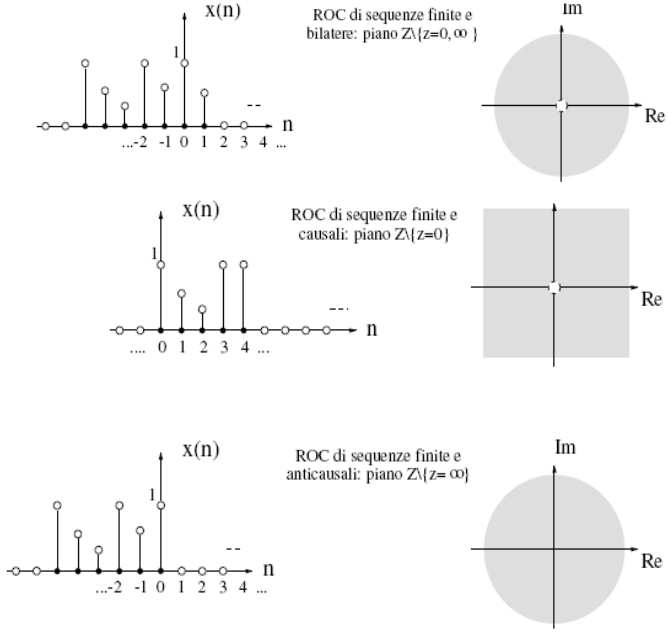
\includegraphics[width=0.6\textwidth]{Lezioni/Immagini/roc}
	\vspace{-40pt}
\end{wrapfigure}

La trasformata converge per qualunque $z$ nel piano complesso, eccetto il punto $z = 0$ se esistono termini del tipo $z^{-k}$ con $k > 0$, e il punto $z = \infty$ se esistono termini del tipo $z^{+k}$ con $k > 0$.

Essendoci polinomi, sia il numeratore che il denominatore potrebbero annullarsi: nel primo caso si chiamano zeri, altrimenti poli. Per individuare i valori si può raccogliere i fattori arrivando all'ordine 1 nel denominatore.

ROC per segnali di durata finita:
\begin{itemize}
	\item ROC per segnali bilateri di durata finita: intero piano complesso $\mathbb{C}$ tranne $[z = 0 \land z = \infty]$;
	\item ROC per sequenze finite e causali: intero piano complesso $\mathbb{C}$ tranne $[z = 0]$;
	\item ROC per sequenze finite e anticausali: intero piano complesso $\mathbb{C}$ tranne $[z = \infty]$.
\end{itemize}
In questo caso i campioni infiniti vengono rappresentati come rapporto finito di polinomi infiniti.

\newpage
\subsection{Poli e zeri}
I poli sono le radici del numeratore e gli zeri sono le radici del numeratore (possono trovarsi anche nelle pulsazioni complesse). Il loro numero è uguale.

 \begin{wrapfigure}{L}{0.4\textwidth}
 	% \vspace{-15pt}
 	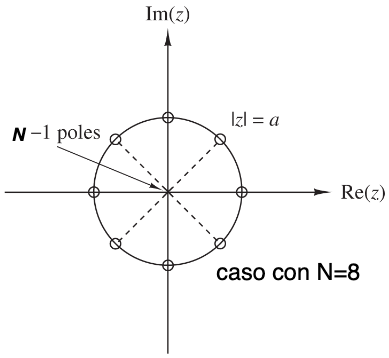
\includegraphics[width=0.4\textwidth]{Lezioni/Immagini/circonferenza}
 	\vspace{-40pt}
 \end{wrapfigure}

Il numero di poli e quello degli zeri corrisponono all'ordine del polinomio che li origina (quindi inizialmente possono essere diversi, ma vengono poi bilanciati con poli/zeri aggiuntivi).
$$X(z) = \frac{1 - \alpha^Nz^{-N}}{1 - \alpha z^{-1}} = z^{-N+1} \frac{z^N - \alpha^N}{z - \alpha}$$

C'è una parte in comune $z = \alpha$ che annulla sia denominatore che numeratore, quindi gli zeri corrispondenti si semplificano e la sequenza resta finita. Ci sono $N - 1$ poli (e zeri) per $z = 0$.

Le radici si posizionano in modo uniforme a intervalli distanti uguali, nelle pulsazioni complesse, su una circonferenza di raggio $\alpha$ (polinomio di ordine $N$, $z^N - \alpha^N$).

\subsection{ROC per sequenze infinite}
Le sequenze $x(n)$ illimitate sono i segnali a tempo discreto che possiedono un supporto temportale illimitato, ma convergono solo in una distinta parte dei piano complesso. 

\begin{wrapfigure}{R}{0.65\textwidth}
	\vspace{-35pt}
	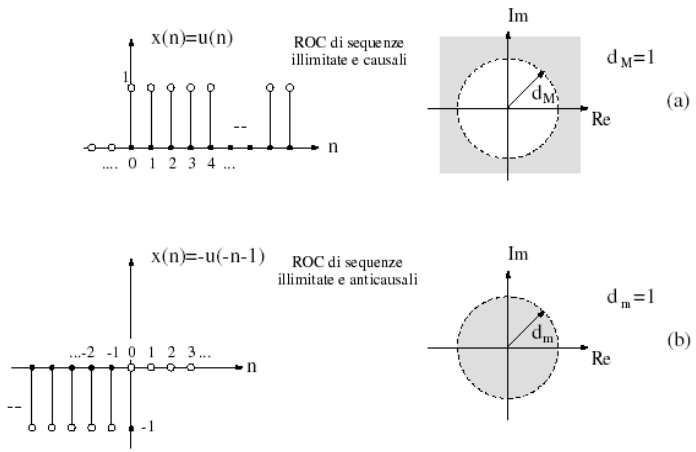
\includegraphics[width=0.65\textwidth]{Lezioni/Immagini/rocinf}
	\vspace{-35pt}
\end{wrapfigure}

Regione di convergenza per sequenze causali: \\
$\abs{z} > d_M$, dove $d_M$ è il modulo del polo più distante dall'origine.

Esempio: sequenza gradino con ROC $\abs{z} > 1$.

Regione di convergenza per sequenze anticausali: \\
$\abs{z} < d_M$, dove $d_M$ è il modulo del polo più vicino all'origine. 

Esempio: sequenza gradino con ROC $\abs{z} < 1$.

Per definizione, la regione di convergenza non può contenere poli. Le sequenze causali, quindi, hanno poli all'esterno della circonferenza, mentre le sequenze anticausali all'interno.

\subsection{Trasformata zeta razionale}
Nei casi pratici di interesse, la funzione $X(z)$ è una funzione razionale di due polinomi: $X(z) = \frac{N(z)}{D(z)}$.
$N(z)$ e $D(z)$ sono due polinomi nella variabile $p_n$ e $p_d$. Scrivendo i due polinomi in forma estesa, si ottiene:
$$X(z) = \frac{\beta_0 + \beta_1z^{-1} + \dots + \beta_{p_n}}{z^{-p_n}}{\alpha_0 + \alpha_1z^{-1} + \dots + \alpha_{p_d}z^{-p_d}}$$
Esprimendo in termini di potenze positive di $z$ e fattorizzando i due polinomi in base alle rispettive radici elementari, si ottiene:
$$X(z) = \frac{\beta_0}{\alpha_0}\big(z^{p_d - p_n}\big) \frac{\prod_{p_n}^{i=1}(z-c_i)}{\prod_{p_d}^{i=1}(z-d_i)}$$
I coefficienti $c_i \forall\ i = 1, \dots, p_n$ sono gli zeri non nulli di $X(z)$, mentre i coefficienti $d_i \forall\ i = 1, \dots, p_n$ sono i poli non nulli di $X(z)$.

Ci sono $p_n - p_d$ poli in $z = 0$ nel caso in cui $p_n > p_d$. \\
Ci sono $p_d - p_n$ poli in $z = 0$ nel caso in cui $p_d > p_n$. 

\section{Analisi dei sistemi}
I sistemi LTI a tempo discreto possono essere descritti da equazioni lineari alle differenze a coefficienti costanti:
$$y(n) = -\alpha_1y(n-1) - \alpha_2y(n - 2) - \dots - \alpha_My(n - M) + \beta_0x(n) + \beta_1x(n - 1) + \dots + \beta_Nx(n - N)$$
Applicando la trasformata di Fourier discreta a ogni termine si ottiene:
$$Y\big(e^{j\omega}\big) = -\alpha_1Y\big(e^{j\omega}\big)e^{-j\omega} - \dots - \alpha_MY\big(e^{j\omega}\big)e^{-j\omega M} + $$
$$ + \beta_0 X\big(e^{j\omega}\big) + \beta_1X\big(e^{j\omega}\big)e^{-j\omega} + \dots + \beta_NX\big(e^{j\omega}\big)e^{-j\omega N}$$
Si ricorda che $F\big(f(x - x_o)\big) = e^{-j2\pi ux_0} F(u)$. Raccogliendo tutti i termini $Y\big(e^{j\omega}\big)$ e $X\big(e^{j\omega}\big)$, si ha:
$$Y\big(e^{j\omega}\big) \big(1 + \alpha_1e^{-j\omega} + \dots + \alpha_Me^{-j\omega M}\big) = X\big(e^{j\omega}\big) \big(\beta_0 + \beta_1e^{-j\omega} + \dots + \beta_Ne^{-j\omega N}\big)$$

Per il teorema della convoluzione, $y(n) = x(n) * h(n) \leftrightarrow Y(e^{j\omega}) = X(e^{j\omega})H(e^{j\omega})$.

La risposta in frequenza $H(e^{j\omega})$ di un sistema LTI espresso tramite le equazioni alla differenze, può essere calcolata come segue:
$$H(e^{j\omega}) = \frac{Y(e^{j\omega})}{X(e^{j\omega})} = \frac{\big(\beta_0 + \beta_1e^{-j\omega} + \dots + \beta_Ne^{-j\omega N}\big)}{\big(1 + \alpha_1e^{-j\omega} + \dots + \alpha_Me^{-j\omega M}\big)}$$
Questo per la relazione che lega trasformata di Fourier e zeta: \\
$\sum_{n=-\infty}^{\infty} x(n)z^{-n} = \sum_{n=-\infty}^{\infty} \big(x(n)\rho^{-n}\big)e^{-j\omega n}$.

La regone di convergenza della funzione $Y(z)$ coincide, nel caso generale, quando non avvengono cancellazioni tra poli e zeri in $X(z)$ e $H(z)$, con l'intersezione tra le regioni delle due funzioni.

Essendo la funzione di trasferimento $H(e^{j\omega})$ razionale, allora anche $H(z)$ lo è, quindi si può esprimere con una funzione razionale del tipo:
$$H(z) = \frac{Y(z)}{X(z)} = \frac{\big(\beta_0 + \beta_1z^{-1} + \dots + \beta_Nz^{-N}\big)}{\big(1 + \alpha_1z^{-1} + \dots + \alpha_Mz^{-M}\big)}$$
Essa corrisponde all'equazione alle differenze, e al caso generale di un sistema LTI.

Un sistema LTI causale e non ricorsivo di tipo FIR ha una funzione di trasferimento del tipo: \\
$H(z) = \beta_0 + \beta_1z^{-1} + \dots + \beta_Nz^{-N}$.

Un sistema LTI causale e puramente ricorsivo di tipo IIR ha una funzione di trasferimento del tipo:
$H(z) = \frac{1}{(1 + \alpha_1z^{-1} + \dots + \alpha_Mz^{-M})}$.

